% Detailed system design. Compile with Tectonic or XeLaTeX.
\documentclass[12pt,letterpaper]{article}
\usepackage[margin=0.8in]{geometry}
\usepackage{fontspec}
\IfFileExists{/System/Library/Fonts/Supplemental/Times New Roman.ttf}{%
  \setmainfont{Times New Roman}[Path=/System/Library/Fonts/Supplemental/,
    Extension=.ttf,UprightFont=*,BoldFont=* Bold,ItalicFont=* Italic,
    BoldItalicFont=* Bold Italic]
  \setmonofont{Times New Roman}[Path=/System/Library/Fonts/Supplemental/,Extension=.ttf]
}{\IfFontExistsTF{Times New Roman}{\setmainfont{Times New Roman}\setmonofont{Times New Roman}}%
  {\setmainfont{Liberation Serif}\setmonofont{Liberation Serif}}}
\usepackage{graphicx}
\usepackage{booktabs,longtable,array,ragged2e}
\usepackage{fancyvrb}
\usepackage{caption}
\usepackage[hidelinks]{hyperref}
\hypersetup{pdftitle={In-Home Assistive Robot: Detailed System Design},
  pdfauthor={Gavin Lamphier; Liam Patel; Austin Heiss}}
\captionsetup{font=small,labelfont=bf,labelsep=period,skip=8pt,hypcap=false}
\setlength{\parindent}{0pt}
\setlength{\parskip}{6pt plus 1pt}
\setlength{\emergencystretch}{2em}
\setlength{\LTpre}{8pt}
\setlength{\LTpost}{10pt}
\renewcommand{\baselinestretch}{1.08}
\newcommand{\field}[1]{\texttt{#1}}
\pagestyle{plain}
\begin{document}
\pagenumbering{gobble}
\begin{titlepage}
\centering
\vspace*{1.2in}
{\LARGE\bfseries In-Home Assistive Robot\par}
\vspace{0.25in}
{\Large Detailed System Design\par}
\vspace{0.12in}
{\large Design D1\par}
\vspace{0.8in}
\begin{tabular}{ll}
Gavin Lamphier & Industrial Design \\[6pt]
Liam Patel & Mechanical Engineering \\[6pt]
Austin Heiss & Computer Science \\[6pt]
\end{tabular}
\vspace{0.55in}
\par October 8, 2026
\vfill
\begin{minipage}{0.84\textwidth}
\textbf{Goal.} Our robot lets an older or disabled adult at home take video calls from a family caregiver and, if they want, have the robot follow them from room to room during the call. The robot stops following as soon as it loses track of them or a safety check fails.
\end{minipage}
\par\vspace{0.16in}{\small AI assisted with drafting and LaTeX formatting.\par}
\vspace*{0.6in}
\end{titlepage}
\pagenumbering{arabic}

\section{Header, scope, and conventions}

\textbf{Goal:} Our robot lets an older or disabled adult at home take video calls from a family caregiver and, if they want, have the robot follow them from room to room during the call. The robot stops following as soon as it loses track of them or a safety check fails.

This document details the \textbf{call server} and \textbf{person tracking}; the resident controls, call manager, audio/video calling, motion control, robot platform, and caregiver app are deferred to D2. We picked these two because the call server holds the data model and person tracking is the computation that breaks following if it is slow or wrong. The APIs in Section 5 also cover where they meet their neighbors (I1, I2, I7, I8, and I14). The caregiver app appears here only as the client of I1 and as a technology choice in Section 6.

\textbf{Figure conventions.} Figure 1 is the only figure. Each blue box is an entity, with its name in bold and its key attributes below it. Each solid line is a relationship; lines have no arrows because they are not data flow. PK marks a primary key, FK a foreign key, and UQ a field covered by a unique index. Cardinality is written at both ends of every line: \textbf{1} means exactly one and \textbf{0..*} means zero or more. The number at a line end tells how many of the entity next to it belong to one record at the other end; for example, the \textbf{0..*} next to Pairing means one robot can have zero or more pairings. The legend repeats this on the figure.

This is a proposed build plan for one resident, one caregiver, and one robot on a clear indoor route (US-01 through US-05). Existing work includes Python simulation/perception prototypes, a consent/following bridge, and JavaScript screen mocks. The call server, database, production sign-in, and iOS companion are proposed integrations, not deployed services. The caregiver app will request/end calls and display outcomes through I1, use I13 for sign-in, and use I12 for media after resident acceptance; it cannot grant itself CALL or FOLLOW permission.

\textbf{Evidence boundary.} Real public-video experiments did not establish sustained selected-person tracking: the initial acquisition failed, and a later same-sample selection lasted only frames 5--7 before loss. Synthetic RGB-D integration suppressed travel requests but failed stationary hold. Some later bounded simulations improved nominal stopping; feedback-loss cases still failed. No physical stopping, calibrated live person-depth, or integrated mobile call has been demonstrated. Time limits are design targets, not measured deployment guarantees.

\section{Data model, the D1 diagram}

The call server uses a relational SQLite database. Figure 1 records account-to-robot enrollment and call outcomes. A pairing permits a caregiver's account to request a call; the resident's separate CALL and FOLLOW permissions remain on the robot and can still deny it (US-02, US-03; I1, I2, I14).

\begin{center}
\begin{minipage}{\linewidth}
\centering
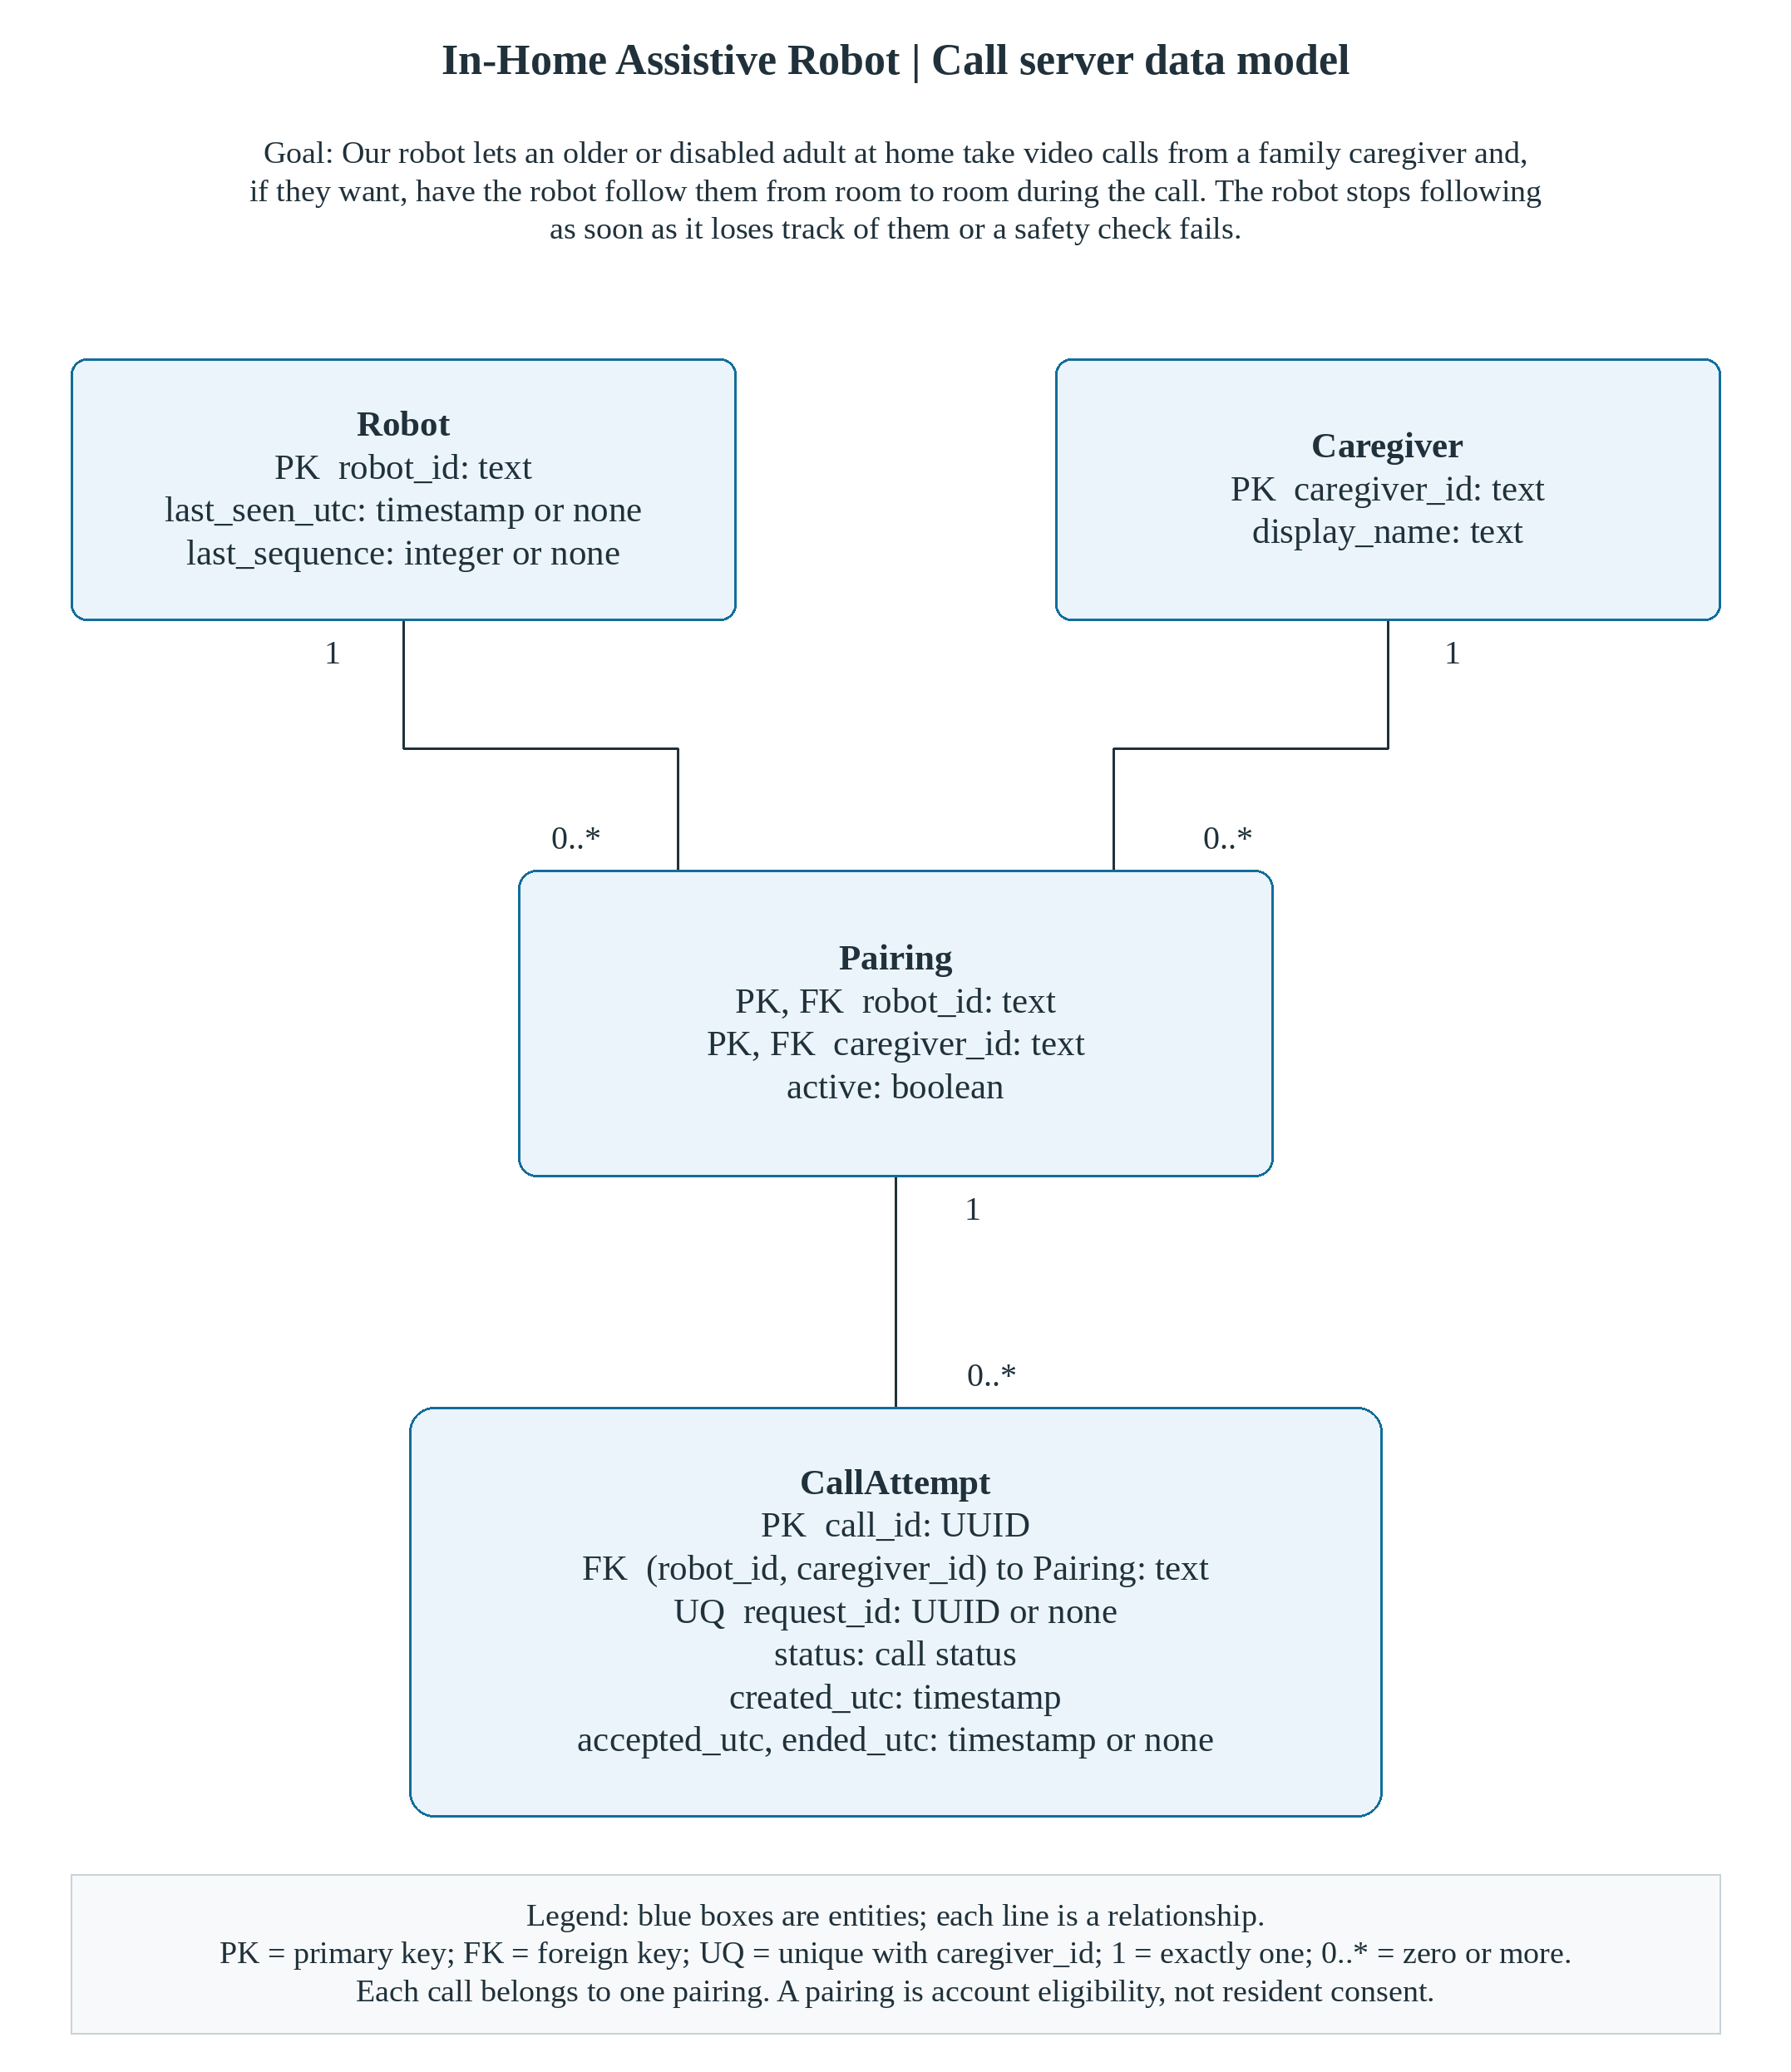
\includegraphics[width=\linewidth,height=0.82\textheight,keepaspectratio]{D1_Data_Model.png}
\captionof{figure}{Call server data model}\label{fig:model}
\end{minipage}
\end{center}

A robot and a caregiver can each have zero or more pairings; each pairing names exactly one of each. One pairing can have zero or more calls, and each call belongs to exactly one pairing through the composite foreign key \field{(robot\_id, caregiver\_id)}. An inactive pairing (\field{active} = false) stays in the database so its old calls keep their owner. Robot stores \field{last\_seen\_utc} and \field{last\_sequence} so the server can tell a fresh heartbeat from a repeated one (I2). We store no audio, video, passwords, access tokens, resident locations, or medical records. \field{accepted\_utc} and \field{ended\_utc} are null until those events happen, and all timestamps are RFC 3339 UTC text. The status values are \field{ringing}, \field{connected}, \field{declined}, \field{no\_answer}, \field{offline}, \field{ended}, and \field{failed}.

\begingroup\small
\begin{longtable}{@{}>{\RaggedRight\arraybackslash}p{0.28\linewidth}>{\RaggedRight\arraybackslash}p{0.68\linewidth}@{}}
\caption{Structural decisions and requirement links}\\
\toprule\textbf{Decision} & \textbf{Reason}\\\midrule\endfirsthead
\toprule\textbf{Decision} & \textbf{Reason}\\\midrule\endhead
\midrule\endfoot\bottomrule\endlastfoot
CallAttempt is an entity & Each attempt needs its own time, status, and owner. A single status field on Robot would erase earlier attempts (US-03). \\
Pairing is an entity & A caregiver and a robot can each be associated with more than one counterpart. The separate pair records that many-to-many relationship and its active/revoked state; it does not replace resident consent (US-02). \\
Pairing to CallAttempt is one-to-many & One attempt belongs to one robot-caregiver pair; that pair can have many attempts. Sharing one attempt among several pairings would make its outcome ambiguous (US-01, US-03). \\
Heartbeat sequence is an attribute of Robot & Only the newest heartbeat matters, so we keep one \field{last\_sequence} value instead of a Heartbeat table that would grow by one row per second. The algorithm compares against it to ignore repeated or out-of-order heartbeats (I2). \\
Keys and indexes & The Robot and Caregiver primary keys and the composite Pairing key support direct lookups. CallAttempt is indexed on \field{(robot\_id, created\_utc)} so the server can find a robot's latest call quickly. \field{(caregiver\_id, request\_id)} has a unique index so a retried start finds the original call instead of making a second one (I1). A partial unique index on \field{robot\_id} for ringing or connected calls stops two active calls on one robot (US-03). \\
Relational store & We chose a relational model in SQLite because the rules above are constraints and transactions, which SQLite enforces for us on a single server. A plain JSON file would make simultaneous updates and uniqueness our problem. Only the call server opens the database file; the robot talks to it over I2. \\
\end{longtable}
\endgroup

\section{Core algorithms}

\subsection*{1. Call attempt and outcome handling}

\textbf{What it is and the problem it solves.} The call server takes a caregiver's request and the robot's replies and turns them into one current outcome for each call. If it gets this wrong, the caregiver could see ``connected'' before the resident has accepted, or a decline could be overwritten by a later message. If it is slow, the caregiver waits on a call that already failed (US-02, US-03; I1, I2, I14).

\textbf{Inputs and outputs.} From the caregiver app (I1): \field{robot\_id}: text, \field{action}: \field{start} or \field{end}, optional \field{request\_id}: UUID, \field{call\_id}: UUID (for end), and a Bearer access token in the request header. From the robot (I2): a heartbeat with \field{sequence}: 64-bit nonnegative integer, or an event with \field{call\_id}: UUID and \field{event}: enum. Output: \field{call\_id}: UUID, \field{status}: call-status enum, and \field{last\_seen}: UTC timestamp or null. A rejected input returns an error code and message, both text. Exact ranges are in Section 5.

\textbf{How it works.} The server checks the token with the sign-in service and then checks for an active pairing. For a new start, it opens one database transaction, looks up the \field{request\_id} if one was sent, checks the robot's last heartbeat, and inserts one CallAttempt. If the robot is offline the call is recorded as OFFLINE; otherwise it is RINGING and the server sends an invite over I2.

From RINGING, the resident's answer has to come through the robot. DECLINED is final. ACCEPTED records \field{accepted\_utc} but the status stays RINGING until the robot reports MEDIA\_CONNECTED; if that does not come within 2 seconds the call becomes FAILED. With no acceptance after 60 seconds the call becomes NO\_ANSWER. The two-second acceptance-to-display target includes network and app time; the server timeout alone does not demonstrate it. A heartbeat only counts if its sequence is greater than \field{last\_sequence}; if no counted heartbeat arrives for 5 seconds, the robot is reported OFFLINE with its last-seen time. ENDED, DECLINED, NO\_ANSWER, OFFLINE, and FAILED are terminal, so reconnecting always means a new call and a new acceptance. Timeouts use the server's monotonic clock, and stored times are UTC for display. On server restart, a transaction closes stored ringing/connected attempts as FAILED with an end time. Every robot then counts as offline until it opens a new authenticated session and sends a heartbeat. A new session retires the old connection and resets its heartbeat sequence baseline, so a robot reboot can start at zero; events from the retired connection are rejected. Calls do not resume automatically.

\textbf{Complexity at our data size.} Each request does a constant number of indexed lookups and one insert or update, so the database work is O(log M) for M stored calls. A planning workload of one robot, one caregiver, and 10 calls a day retained for 30 days gives M = 300; the rate and retention period are assumptions to confirm. At 100 times that history (M = 30,000), log-base-2 M grows from about 9 to 15. These illustrate logarithmic growth, not SQLite page reads, measured comparisons, or latency. Network checks and write contention still need measurement. Heartbeats are the part that grows: 1 write per second for one robot becomes about 100 writes per second for 100 robots. SQLite allows one writer at a time [2], so that is the first thing we would benchmark before scaling up, and the reason PostgreSQL is our fallback in Section 6.

\textbf{Why this approach.} We compared three options. (1) Keeping only the latest status in a file or a Robot column is simpler, but it loses call history (US-03) and cannot settle two starts that arrive together. (2) Letting the robot own the call state and the server only relay messages fails when the robot goes offline: the caregiver would get no answer at all, which is exactly the case US-03 cares about. (3) A server-side state machine in a database transaction, with a partial unique index for one active call per robot, keeps history, handles the offline case, and lets the database reject races. We chose (3). We also push status over a secure WebSocket rather than having the app poll every second, which would add up to a second of delay and constant load for no new information.

\textbf{Edge cases.}
\begin{itemize}\setlength{\itemsep}{2pt}
\item \emph{Empty or malformed input:} missing fields, bad UUIDs, or unknown fields return 400 INVALID\_REQUEST and change nothing (I1).
\item \emph{Duplicates:} a repeated start with the same caregiver, \field{request\_id}, and robot returns the original call. A repeated robot event or heartbeat does not change a terminal call or refresh last-seen time (I2).
\item \emph{Ties and races:} if two starts for one robot arrive together, the partial unique index lets one insert win and the other gets 409 ACTIVE\_CALL. If an acceptance arrives after the 60-second deadline, arrival time decides and the call stays NO\_ANSWER.
\item \emph{Retry ID misuse:} a \field{request\_id} reused for a different robot returns 409 REQUEST\_CONFLICT.
\item \emph{Failures:} if the sign-in service or database is down the server returns 503 and never grants access by default (I14). A missing media confirmation or heartbeat never turns into CONNECTED.
\end{itemize}

\subsection*{2. Selected-person tracking and loss handling}

\textbf{What it is and the problem it solves.} This runs on the robot. It keeps track of the one person the resident selected and gives motion control their distance and direction. If it is wrong, the robot can follow a visitor; if it is slow, the robot steers toward where the resident used to be. So it must stop giving a usable position whenever its data is stale, missing, ambiguous, or no longer allowed (US-01, US-02, US-04; I7, I8, I9).

\textbf{Inputs and outputs.} Inputs are the target ID, CALL/FOLLOW gates, permission generation, frame times, detector candidates, an optional selected-instance mask, and a calibrated depth-projection result for that same target, frame, and generation. Pixel positions and projected optical depth are finite floats; timestamps/generation are nonnegative 64-bit integers. Output is an I7 TrackRecord containing target ID, valid/unavailable status, range/bearing or null, capture/expiry times, a reason, coordinate frame, and a false motion-authorization flag. Section 5 defines the types. This is an offline candidate contract; conversion to a qualified robot-frame position remains integration work.

\textbf{How it works.} After accepting a call and pressing Follow, the resident picks one visible person on the screen. On each new frame:
\begin{enumerate}\setlength{\itemsep}{2pt}
\item \emph{Gate.} Reject the frame if permission is off, its timestamp is in the future or more than 200 ms old, image/depth capture times differ by more than 50 ms, or calibration evidence is missing. The 200 ms freshness gate and 0.8 detection filter come from the existing prototype; the 50 ms skew and association/range thresholds below remain provisional design values.
\item \emph{Associate.} Keep candidates with confidence at least 0.8. For a new explicit selection, use the named candidate without a prior-box match; reject overlapping ambiguous candidates. On later frames, compare intersection over union (IoU) with the last selected box. Accept a best IoU of at least 0.30 only if it beats the second best by more than 0.15. If another kept box overlaps the winner by 0.50 IoU or more, report ambiguity. These geometric tests do not establish identity assurance.
\item \emph{Measure.} Require the exact selected-person mask and a candidate-status result from the calibrated projection adapter, bound to the selected target, frame, and generation. That adapter must check per-zone rays, radial range-error intervals, camera intrinsics/extrinsics, timing/pose uncertainty, and independent clear visibility. The whole projected zone envelope must lie inside the selected mask; a centre pixel or a boolean registration flag is insufficient. Reject inconsistent depth rather than selecting a convenient nearest cluster. Require at least three admitted zones whose entire depth intervals lie in the provisional 0.2--4.0 m domain. For offline inspection, \field{range\_m} is median RGB optical-axis Z, distinct from raw radial ToF range and robot stopping clearance. Bearing uses arctan((mean projected x - \field{cx\_px}) / \field{fx\_px}) in degrees, positive right.
\item \emph{Publish.} Recheck the permission generation and expiry at publication. Emit a VALID offline candidate only while fresh, with \field{motion\_authorized=false}; otherwise report UNAVAILABLE. Current projection experiments do not grant movement authority.
\end{enumerate}
If any step fails, publish UNAVAILABLE with null range and bearing, latch the loss, and wait for the resident to select and press Follow again. A watchdog publishes the loss even if no new frame arrives. Motion control must reject these motion-disconnected candidates. A future movement path also needs validated identity, a calibrated transform to the robot frame, independent clearance, freshness, resident permission, and qualified stopping. A zero travel request is not a demonstrated physical stop; the recorded feedback-loss failures remain unresolved.

\textbf{Complexity at our data size.} For N candidates and Q already-admitted depth zones, box association is O(N) and a standard-library median sort is O(Q log Q), with O(Q) extra memory [12]. A planning case of 5 candidates and at most 2,268 zones gives N + Q log\textsubscript{2} Q about 25,300; 100 times the candidates (500) gives about 25,800. These are values of a scaling expression, not counted instructions or measured milliseconds. Camera transport, detector inference, mask construction, full-footprint projection/visibility checks, and control are excluded from this bound and must be budgeted separately. The matched blank-image Mask R-CNN CPU rerun measured about 2.82 s median, excluding the rest of that pipeline; it demonstrates a timing gap rather than person accuracy or a prediction of Pi/Jetson speed.

\textbf{Why this approach.} Nearest-person following could choose a visitor (US-04), so it is rejected. ByteTrack and appearance-based diagnostics have also been explored: raw track IDs continued beyond the selected-target wrapper's loss, while OSNet did not establish sustained selected identity. Neither result permits automatic reacquisition. The proposed baseline therefore retains explicit selection, conservative box association, and a latched loss (US-02, US-04). IoU is an association aid, not proof that two boxes contain the same person. Real identity continuity and masks/depth remain release blockers.

\textbf{Edge cases.}
\begin{itemize}\setlength{\itemsep}{2pt}
\item \emph{Empty input:} no candidates, no mask, or fewer than three valid depth points gives UNAVAILABLE with reason LOST, NO\_MASK, or NO\_DEPTH (I7).
\item \emph{Duplicates:} a repeated \field{frame\_id} returns DUPLICATE and does not extend the old expiry; duplicate candidate IDs return INVALID\_INPUT.
\item \emph{Ties:} two candidates within 0.15 IoU of each other, or overlapping by 0.50 or more, give AMBIGUOUS rather than a guess.
\item \emph{Out of order or stale:} an older frame can never replace a newer result; anything older than 200 ms gives STALE.
\item \emph{Permission change:} Stop, Privacy, or a new generation during processing means the result is thrown away, so a frame computed before Stop cannot restart following (I8).
\item \emph{Known gap:} two people swapping places in the same spot can fool a box tracker. We will test this case directly.
\end{itemize}

\section{Build-versus-reuse decisions}

The table separates existing experimental work from proposed integrations. The team-code license is undecided. Library maturity, base license, and intended fit have been reviewed; actual deployment performance, pinned versions, dependency notices, and model/dataset rights still need verification. The resident permission model should reuse the existing consent/following bridge, rather than create a second consent state machine.

\begingroup\small
\setlength{\tabcolsep}{4pt}
\begin{longtable}{@{}>{\RaggedRight\arraybackslash}p{0.17\linewidth}>{\RaggedRight\arraybackslash}p{0.08\linewidth}>{\RaggedRight\arraybackslash}p{0.16\linewidth}>{\RaggedRight\arraybackslash}p{0.15\linewidth}>{\RaggedRight\arraybackslash}p{0.36\linewidth}@{}}
\caption{What the team builds and reuses}\\
\toprule\textbf{Piece} & \textbf{Build or reuse} & \textbf{Library or service} & \textbf{License} & \textbf{Reason (maturity, license, performance, fit)}\\\midrule\endfirsthead
\toprule\textbf{Piece} & \textbf{Build or reuse} & \textbf{Library or service} & \textbf{License} & \textbf{Reason (maturity, license, performance, fit)}\\\midrule\endhead
\midrule\endfoot\bottomrule\endlastfoot
Call outcome state machine and pairing rules & Build & None & Team code & Build the call-outcome and pairing rules for US-03; integrate the existing resident consent bridge for US-02. The server is not deployed. \\
Relational storage & Reuse & SQLite & Public domain [1] & Transactions and partial indexes fit one server; load tests, backups, and dependency notices remain necessary [2]. \\
HTTP and WebSocket server & Reuse & FastAPI on Uvicorn & MIT / BSD-3-Clause [3,4] & Maintained, permissive Python stack; async I/O is available, but blocking database/auth work must not block heartbeats. \\
Request validation & Reuse & Pydantic (used by FastAPI) & MIT [17] & Set \field{extra='forbid'}, strict scalar types, and finite/range validators; the defaults do not enforce this entire contract [21]. \\
Sign-in and accounts & Reuse & Keycloak & Apache-2.0 [5] & Mature OIDC service candidate; avoids custom passwords. Introspection timing and deployment are unmeasured. \\
Token verification on the server & Reuse & Authlib & BSD-3-Clause [18] & OIDC/OAuth client candidate; verify asynchronous introspection and error mapping with the pinned release before integration. \\
Timestamps and UUIDs & Reuse & Python \field{datetime} and \field{uuid} & PSF [8] & Standard library, so nothing to install; parsing RFC 3339 by hand is a common source of bugs. \\
Selection, IoU matching, and loss latch & Build & NumPy for array math & Team code; NumPy BSD-3-Clause [19] & Project-specific rules for US-04; NumPy is an optional array tool, not a demonstrated latency guarantee. \\
Person detector and masks & Reuse & TorchVision Mask R-CNN (first candidate) & BSD-3-Clause code [6]; weight terms checked separately & Existing offline mask adapter; sampled CPU timings exceed 200 ms. SSDLite is a separate box-only baseline and cannot replace selected-instance masks. \\
Calibrated RGB--ToF projection & Build / reuse prototype & Existing standard-library Python contract & Team code; PSF runtime [8] & Reuse synthetic geometry checks; actual calibration, visibility evidence, sensor data, and movement integration are absent. \\
Simulation & Reuse & MuJoCo & Apache-2.0 [7] & Existing simulation/training tool; bounded successes and failed stopping/latency cases do not establish transfer to hardware. \\
Caregiver iOS app & Build & Swift and SwiftUI & Apache-2.0 with runtime exception; Apple SDK terms [14,15] & Native iOS UI fits the requested companion; build on Austin's prior SwiftUI work. Real calling, accessibility, and background behavior remain untested. \\
\end{longtable}
\endgroup

\section{API contract}

This section specifies I1 and I2 on the call server and I7/I8 for person tracking. Rules that apply everywhere: JSON field names are case-sensitive and unknown fields are rejected. UUIDs are canonical 36-character strings, and timestamps are RFC 3339 UTC strings such as \field{2026-10-02T14:30:00Z}. Every caregiver request carries its token in an \field{Authorization: Bearer <token>} header (1--4096 characters), never in the body, and the server never stores or logs it. Every HTTP error contains an \field{error} object with \field{code} and \field{message}, both text, and no success fields. Map framework validation failures to the specified 400 response; do not leak tokens or raw input in error logs. A pairing makes an account eligible to call; it is not the resident's permission.

\begingroup\small
\setlength{\tabcolsep}{4pt}
\begin{longtable}{@{}>{\RaggedRight\arraybackslash}p{0.22\linewidth}>{\RaggedRight\arraybackslash}p{0.2\linewidth}>{\RaggedRight\arraybackslash}p{0.2\linewidth}>{\RaggedRight\arraybackslash}p{0.32\linewidth}@{}}
\caption{API summary}\\
\toprule\textbf{Endpoint or method} & \textbf{Inputs} & \textbf{Output} & \textbf{Errors (code: when)}\\\midrule\endfirsthead
\toprule\textbf{Endpoint or method} & \textbf{Inputs} & \textbf{Output} & \textbf{Errors (code: when)}\\\midrule\endhead
\midrule\endfoot\bottomrule\endlastfoot
POST /v1/\allowbreak call-commands (I1) & Bearer token; \field{robot\_id}, \field{action}, optional \field{request\_id}, \field{call\_id} for end & CallStatus; 202 for a new ringing call, 200 otherwise & 400: bad input; 401: bad or expired token; 403: not paired; 404: unknown robot or call; 409: active call or retry ID conflict; 503: sign-in or database down \\
GET /v1/\allowbreak calls/\allowbreak\{call\_id\} (I1) & Bearer token; \field{call\_id} in path & CallStatus, 200 & 400: bad UUID; 401; 403; 404; 503 \\
WSS /v1/\allowbreak calls/\allowbreak\{call\_id\}/\allowbreak updates (I1) & Bearer token on connect; \field{call\_id} in path & CallStatus on every change & Close 1008: bad or unauthorized token; close 1011: server failure \\
WSS /v1/\allowbreak robots/\allowbreak\{robot\_id\}/\allowbreak session (I2) & Robot token; heartbeat and event frames & Invite and cancel frames & Error frame INVALID\_MESSAGE or STALE\_CALL; close 1008: bad robot identity; close 1011: storage failure \\
trackSelected (I7, I8) & Frame, candidates, depth, gates, prior state & TrackRecord & TrackError INVALID\_INPUT, NO\_SELECTION, or DUPLICATE \\
\end{longtable}
\endgroup

CallStatus is \field{\{call\_id: UUID, status: call-status enum, last\_seen: UTC timestamp or null\}}.

\subsection*{Call server: I1}

\textbf{POST /v1/call-commands.} The body is a JSON object with these fields:

\begingroup\small
\begin{longtable}{@{}>{\RaggedRight\arraybackslash}p{0.24\linewidth}>{\RaggedRight\arraybackslash}p{0.72\linewidth}@{}}
\toprule\textbf{Input} & \textbf{Type, requirement, and valid values}\\\midrule\endfirsthead
\toprule\textbf{Input} & \textbf{Type, requirement, and valid values}\\\midrule\endhead
\midrule\endfoot\bottomrule\endlastfoot
\field{robot\_id} & Required text, 1--64 characters, letters, numbers, hyphen, or underscore; an enrolled robot. \\
\field{action} & Required enum: \field{start} or \field{end}. \\
\field{request\_id} & Optional UUID or null for start; when supplied, unique per caregiver. It must be omitted or null for end. \\
\field{call\_id} & Required UUID for end; omitted or null for start. It must identify a call for the given robot and authenticated caregiver's pairing. Ending a terminal attempt returns its existing result. \\
\end{longtable}
\endgroup

\textbf{Success, HTTP 202 or 200:} a CallStatus object. A new start to an online robot returns 202 with \field{ringing}; a start to an offline robot returns 200 with \field{offline}. A retry or an end returns 200 with the current or final status. \field{ringing} does not mean the resident accepted; only \field{connected} does.

\textbf{Errors:} 400 INVALID\_REQUEST for invalid types, ranges, or conditional fields; 401 UNAUTHENTICATED for an invalid/expired token; 403 NOT\_PAIRED for a valid account without an active pairing; 404 NOT\_FOUND for an unknown robot or call; 409 ACTIVE\_CALL or REQUEST\_CONFLICT for a second active call or a retry ID reused with different input; 503 SERVICE\_UNAVAILABLE if the identity service or database is unavailable. The caller may retry a 503, preferably with the same request ID; it must not treat a rejected request as a connected call.

\textbf{GET /v1/calls/\{call\_id\}.} Input is a required UUID path parameter plus the Bearer header. The caller must own the active pairing for the call. HTTP 200 returns a CallStatus. Errors: 400 INVALID\_REQUEST for a bad UUID, 401 UNAUTHENTICATED, 403 NOT\_PAIRED, 404 NOT\_FOUND, and 503 SERVICE\_UNAVAILABLE.

\textbf{WSS /v1/calls/\{call\_id\}/updates.} The app opens this socket with the same Bearer header. After the token and pairing checks, the server sends a CallStatus right away and again whenever the status or last-seen time changes; the client sends nothing. The server closes with code 1008 for a missing, invalid, or unauthorized token and 1011 for a sign-in or storage failure. If the socket drops, the app shows that it lost contact and can call GET after reconnecting; a dropped socket never means the call connected.

\begin{minipage}{\linewidth}
\textbf{Example I1 request and response:}
\begin{Verbatim}[fontfamily=tt,fontsize=\small]
POST /v1/call-commands
Authorization: Bearer eyJhbGciOi...
Content-Type: application/json

{"robot_id": "home-robot-01", "action": "start",
 "request_id": "e5c7cb31-343c-4fb8-a632-054e84465d24"}

HTTP/1.1 202 Accepted
Content-Type: application/json

{"call_id": "f34f4e06-d38c-4dbd-a9b1-d11650d06599",
 "status": "ringing", "last_seen": "2026-10-02T14:30:00Z"}

HTTP/1.1 409 Conflict      (new request_id; another call is active)
{"error": {"code": "ACTIVE_CALL",
           "message": "This robot already has an active call."}}
\end{Verbatim}
\end{minipage}

\subsection*{Robot session: I2}

\textbf{WSS /v1/robots/\{robot\_id\}/session.} The path has the same robot ID rules as I1. An authenticated robot service token in the Bearer header is required; its subject must match the enrolled robot. Robot-to-server JSON frames are a heartbeat with \field{type:"heartbeat"} and integer \field{sequence}, sent every second, or an event with \field{type:"event"}, UUID \field{call\_id}, and \field{event}. Sequence ranges from zero to 2\textsuperscript{63}-1; event is ACCEPTED, DECLINED, MEDIA\_CONNECTED, MEDIA\_FAILED, or ENDED. Server-to-robot JSON frames are an invite with \field{type:"invite"}, UUID \field{call\_id}, text \field{caller\_name}, and timestamp \field{expires\_utc}; or a cancel with \field{type:"cancel"}, UUID \field{call\_id}, and \field{reason}. Reason is ENDED, NO\_ANSWER, OFFLINE, or FAILED. Names are 1--80 characters. Sequence is scoped to the current authenticated session: opening a new session retires the old socket and clears \field{last\_sequence}; subsequent heartbeats must increase it. Old-session messages cannot refresh \field{last\_seen\_utc} or revive a call.

A malformed or invalid event gets \field{\{type:"error", code:"INVALID\_MESSAGE" or "STALE\_CALL"\}}; it cannot change a terminal call. The server closes with WebSocket code 1008 for a bad robot identity or repeated invalid messages and 1011 for an internal storage failure. When the session drops, the server marks the robot offline after 5 seconds, and the robot ends any call in progress (D0, I2).

\subsection*{Person tracking method: I7 and I8}

\textbf{trackSelected(input) -> TrackRecord or TrackError.} This is an in-process function call on the robot, not an HTTP endpoint. Every field below is required unless marked optional. Time values are integer milliseconds in one robot monotonic clock domain, from 0 to 2\textsuperscript{63}-1.

\begingroup\small
\begin{longtable}{@{}>{\RaggedRight\arraybackslash}p{0.24\linewidth}>{\RaggedRight\arraybackslash}p{0.72\linewidth}@{}}
\toprule\textbf{Input} & \textbf{Type, requirement, and valid values}\\\midrule\endfirsthead
\toprule\textbf{Input} & \textbf{Type, requirement, and valid values}\\\midrule\endhead
\midrule\endfoot\bottomrule\endlastfoot
Selection and gates & \field{target\_id}: text, 1--64 characters; \field{call\_accepted} and \field{follow\_allowed}: booleans; \field{generation}: nonnegative integer. \\
Time and frame & \field{now\_ms}, \field{frame\_id}, \field{capture\_ms}: nonnegative integers. Image \field{width} and \field{height}: positive integers, each at most 1920, with width times height at most 2,073,600 pixels. \\
Candidates & Array of 0--500 records: \field{candidate\_id} is unique text of 1--64 characters; \field{box} is [left, top, right, bottom] in integer pixel coordinates with positive area; left/top are inclusive, right/bottom exclusive, all within image bounds. \field{confidence} is a finite number in [0,1]. \field{mask} is an optional image-sized boolean array. \\
Depth projection & Required record: \field{target\_id}, \field{candidate\_id} (text, 1--64 characters), \field{frame\_id}, \field{generation}, and \field{capture\_ms} (nonnegative integers); these must match the selected observation. \field{status}: candidate/not\_observed/uncertain; \field{source}: synthetic/offline/hardware. \field{points}: 0--2,268 already-admitted records with finite pixel \field{x}, \field{y}, positive finite \field{optical\_z\_m}, and \field{z\_interval\_m}: two ordered finite positive bounds enclosing that depth. \\
Calibration & \field{fx\_px}: finite number greater than zero and at most 100,000; \field{cx\_px}: finite number from zero inclusive to width exclusive, in pixels for the rectified RGB image. \field{calibration\_id}: text, 1--64 characters, naming the validated revision for this image mode. The upstream adapter also needs measured zone rays, intrinsics/extrinsics, bounded reprojection/range error, synchronized capture times, and per-zone clear visibility; its validated calibration revision must match the frame mode. Nominal field of view is insufficient. \\
Selection state & Optional \field{selected\_candidate\_id}: text or null, required for a new explicit selection. Optional \field{prior}: null or a record with \field{generation}, \field{last\_frame\_id} (nonnegative integers), \field{last\_box} (four in-bounds pixel integers), and \field{loss\_latched} (boolean). \\
\end{longtable}
\endgroup

New selection requires a fresh resident Follow action, a selected candidate, and either no prior state or a generation greater than the prior generation. A latched loss cannot be cleared by later frames alone. The tracker atomically updates its per-target prior state when processing a frame; the next call receives that state. Duplicate frames do not update it.

\textbf{TrackRecord:} fields are \field{target\_id}: text, \field{tracking\_status}: valid/unavailable, \field{range\_m} and \field{bearing\_deg}: finite number or null, \field{capture\_ms} and \field{expires\_ms}: integer milliseconds, \field{reason}: enum, \field{range\_frame}: constant \field{rgb\_optical\_z}, and \field{motion\_authorized}: constant false. Range is median RGB optical-axis Z in metres; bearing is in degrees, positive right. It is not a robot-frame separation or clearance. Valid means an offline candidate with reason OK, expiring by capture + 200 ms; it never grants movement. Unavailable has null range/bearing and reason CONSENT\_OFF, STALE, AMBIGUOUS, LOST, NO\_MASK, NO\_DEPTH, or BAD\_CALIBRATION. Missing calibration gives BAD\_CALIBRATION; not\_observed, uncertain, or missing visibility gives NO\_DEPTH. Stop or a generation change invalidates earlier output immediately. A qualified movement interface requires separate base-frame conversion, identity/clearance checks, and physical validation in D2; it cannot reinterpret this offline range as a robot-frame command.

\textbf{TrackError:} \field{\{code:enum, message:text\}}. INVALID\_INPUT covers missing fields, invalid bounds or duplicate IDs; NO\_SELECTION covers a missing required resident selection; DUPLICATE covers an already processed frame. INVALID\_INPUT and NO\_SELECTION make the caller request a stop. DUPLICATE must not extend the prior record's expiry; the watchdog requests a stop when freshness expires, even if no new method call arrives. The proposed integration serializes permission-generation checks with publication; this atomic cross-component behavior still needs testing. Offline bridge tests alone do not establish it on hardware.

\textbf{Versioning.} The HTTP and WebSocket APIs are versioned by the \field{/v1} path prefix and the tracking method by a version constant in its module; removing or renaming a field, changing a type, unit, required input, status meaning, or error behavior is a breaking change that requires \field{/v2}, while adding an optional output field is not breaking (adding an input field is, because v1 rejects unknown inputs).

\section{Technology choices with justification}

Each paragraph covers team skill fit, licensing, community support, performance, and cost/hosting. These are proposed selections for review; unmeasured capacity, prices, and hosting allowances are not established facts.

\textbf{Database: SQLite.} \emph{Skill:} Python is already used for simulation and perception; the team will still need to implement the SQL schema and migrations. \emph{License:} SQLite's core is public domain, with dependency and deployment notices checked separately [1]. \emph{Community:} official documentation covers transactions, indexing, and deployment [2]. \emph{Performance:} one server is a reasonable starting design, but neither one-robot latency nor 100-robot write contention has been benchmarked. \emph{Cost and hosting:} no database license fee, but durable storage, backups, and administration require an approved host. \emph{Alternative:} PostgreSQL adds an independently operated database service and is the candidate if measured write contention or multi-host deployment warrants it.

\textbf{Backend: Python with FastAPI on Uvicorn.} \emph{Skill:} existing Python experiments provide relevant experience; JavaScript screen mocks are a separate existing code path. \emph{License:} Python PSF, FastAPI MIT, and Uvicorn BSD-3-Clause [3,4,8]. \emph{Community:} both server projects have maintained official documentation. \emph{Performance:} asynchronous I/O can overlap network waits, provided database and authentication work do not block the event loop; a worker count or two-second response guarantee cannot be chosen without measurements. \emph{Cost and hosting:} the software has no license fee; compute, monitoring, and integration still cost resources. \emph{Alternative:} Node.js/Express would use the team's JavaScript experience, but Python keeps the initial server aligned with the simulation/perception tooling.

\textbf{Caregiver front end: iOS app in Swift and SwiftUI.} \emph{Skill:} Austin's prior Swift/SwiftUI app work supports the choice, with Gavin proposed to design the screens. The robot companion itself is not implemented. \emph{License:} Swift is Apache-2.0 with a runtime exception; Apple SDK and team-code terms are separate [14,15]. \emph{Community:} Apple documentation and Swift forums support development; VoiceOver and text sizing still need app-specific tests [16]. \emph{Performance:} foreground call requests and status updates are the initial target. Incoming background calls would need a separately designed APNs/PushKit/CallKit path; no locked-phone ringing or hardware-encoder result has been demonstrated [20]. \emph{Cost and hosting:} a free developer account supports own-device testing; wider distribution may need the \$99/year program, plus a Mac/iPhone and backend hosting [15]. \emph{Alternative:} a browser companion remains a cross-platform option; the requested iOS direction motivates native development, not an untested claim that it solves notification reliability.

\textbf{Identity and messaging: Keycloak, HTTPS, and secure WebSocket.} \emph{Skill:} Python integration is plausible, but production Keycloak operation is not recorded; Austin is the proposed integration owner. \emph{License:} Keycloak Apache-2.0, with Authlib BSD-3-Clause as a client candidate [5,18]. \emph{Community:} official OIDC documentation supports integration [9]. \emph{Performance:} token introspection adds a network operation; its delay, resource footprint, and effect on heartbeats are unmeasured. \emph{Cost and hosting:} no software license fee, but identity storage and operations may need a separate service or a larger host; resource sizing remains to be measured. \emph{Alternative:} managed identity such as Firebase Authentication could reduce administration, but introduces provider terms and costs to evaluate; no provider is deployed.

\textbf{On-robot perception and hardware: Python/TorchVision, host to be selected.} \emph{Skill:} existing offline detector and projection work supports this software direction. \emph{License:} TorchVision/PyTorch base code and bundled dependencies have separate notices; dataset/weight rights remain to be resolved [6,13]. \emph{Community:} official TorchVision, ST, and Raspberry Pi documentation provide supported integration references [6,10,22]. \emph{Performance:} SSDLite is box-only; the measured Mask R-CNN CPU baseline misses 200 ms. Neither Pi 5 nor Jetson performance has been measured. The purchased/shipped VL53L9CXV0VE/1 is a bare depth component, not an RGB-D USB device; carrier, host, real frames, calibration, and power integration remain unverified. A Pi 5 candidate has two shared camera/display ports, so RGB CSI + ToF MIPI + DSI display needs a different verified route [10]. \emph{Cost and hosting:} board variant, carrier, camera, display, storage, power and integration prices need quotes; no replacement build budget is approved. \emph{Alternative:} a Jetson is an evaluation candidate if compute needs justify it, without a promised speedup or automatic hardware switch.

\textbf{Hosting: proposed Ubuntu Server VM.} \emph{Skill:} public-server operating experience is not documented; Austin is the proposed deployment owner. \emph{License:} Ubuntu comprises packages with distinct licenses [11]. \emph{Community:} official platform and server-project deployment documentation are available. \emph{Performance:} test the complete server, identity service, and any media relay against heartbeat and call targets before choosing RAM or worker counts. \emph{Cost and hosting:} provider, VM size, persistent disk, backups, TLS operation, relay traffic, and monthly allowance remain unapproved. \emph{Alternative:} a laptop can support local integration, but remote reachability and availability require separate validation.

\subsection*{Source notes}
\footnotesize
[1] \href{https://www.sqlite.org/copyright.html}{SQLite copyright and public-domain core};
[2] \href{https://www.sqlite.org/whentouse.html}{SQLite deployment and single-writer guidance};
[3] \href{https://github.com/fastapi/fastapi}{FastAPI project and license};
[4] \href{https://github.com/encode/uvicorn}{Uvicorn project and license};
[5] \href{https://github.com/keycloak/keycloak}{Keycloak project and license};
[6] \href{https://github.com/pytorch/vision}{TorchVision project, code license, and weight notice};
[7] \href{https://github.com/google-deepmind/mujoco}{MuJoCo project and license};
[8] \href{https://docs.python.org/3/license.html}{Python license};
[9] \href{https://www.keycloak.org/securing-apps/oidc-layers}{Keycloak OIDC endpoints};
[10] \href{https://www.raspberrypi.com/documentation/computers/sbcs.html}{Raspberry Pi connector documentation};
[11] \href{https://ubuntu.com/legal/intellectual-property-policy}{Ubuntu package and license policy};
[12] \href{https://docs.python.org/3/library/statistics.html}{Python standard-library median};
[13] \href{https://github.com/pytorch/pytorch/blob/main/pyproject.toml}{PyTorch code and bundled dependency licenses};
[14] \href{https://www.swift.org/legal/license.html}{Swift license};
[15] \href{https://developer.apple.com/programs/}{Apple developer tools, testing, and distribution};
[16] \href{https://developer.apple.com/documentation/SwiftUI/Accessibility-fundamentals}{SwiftUI accessibility fundamentals};
[17] \href{https://github.com/pydantic/pydantic}{Pydantic project and license};
[18] \href{https://github.com/authlib/authlib}{Authlib project and license};
[19] \href{https://numpy.org/doc/stable/license.html}{NumPy license};
[20] \href{https://developer.apple.com/documentation/pushkit/responding-to-voip-notifications-from-pushkit}{Apple incoming VoIP notification requirements};
[21] \href{https://docs.pydantic.dev/latest/api/config/}{Pydantic validation configuration};
[22] \href{https://www.st.com/en/imaging-and-photonics-solutions/vl53l9cx.html}{ST VL53L9CX component specifications}.

\normalsize
\end{document}
